In the previous chapter, the author evaluated the feasibility of the proposed load balancer in 1Gbps network.
The author verified that the proposed load balancer has sufficient throughput in 1 Gbps network.
In this chapter, the author shows that the proposed load balancer has sufficient throughput in 10Gbps network.
The author also discusses how to improve the performance levels in faster networks, e.g., 100 Gbps and finds that there are rooms for improvements in both the container network and the software load balancer itself.
Although these should be explored further in the future work, the author presents preliminary experimental results of a novel software load balancer using eXpress Data Plane (XDP) technology.



\section{Throughput measurement in 10G network}

In order to evaluate the performance levels of the proposed load balancer in a 10 Gbps network environment, the author carried out throughput measurements.
Table~\ref{tab:hw_sw_spec_10g} summarizes the hardware and software specification used in the experiment.
Bare metal servers with Intel X550 network card was used.
The X550 NIC has a maximum of 64 rx-queues, and 16 of them are activated by the driver at the boot time since there are 16 logical CPUs.
The setting \enquote{ (RSS, RPS)=(on, off)} is used because interrupts from each of 16 rx-queues can be assigned to separate logical cores.
As a result, packet processing is distributed to all of the 16 logical cores, which results in the best performance in most of the cases.
The host-gw mode is used as the backend mode of the flannel overlay network.

\begin{table}[h]
  \centering
  \begin{minipage}{0.9\columnwidth}
    \begin{lstlisting}[frame=lines,breaklines=true,basicstyle=\small\ttfamily]
 [Hardware Specication]
   CPU: Xeon E5-2450 2.10GHz x 8 (with Hyper Threading)
   Memory: 32GB
   NIC: Intel X550 with 64 rx-queues (16 activated), 10 Gbps
   (Node x 6, Load Balancer x 1, Client x 1))

 [Node Software]
   OS: Debian 9.5, linux-4.16.8
   Kubernetes v1.5.2
   flannel v0.7.0
   etcd version: 3.0.15

 [Container Software]
   Keepalived: v1.3.2 (12/03,2016)
   nginx : 1.15.4 (web server)
    \end{lstlisting}
  \end{minipage}

  \par\bigskip
  \centering
  \begin{minipage}{0.9\columnwidth}
    \caption[Hardware and software specifications for 10 Gbps experiment]{
      Hardware and software specifications for 10 Gbps experiment.
      There are 16 rx-queues activated for the NIC, to match the number of logical CPUs.
    }
    \label{tab:hw_sw_spec_10g}
  \end{minipage}
\end{table}

\begin{figure}[h]
  \begin{subfigure}[t]{\columnwidth}
    \centering
    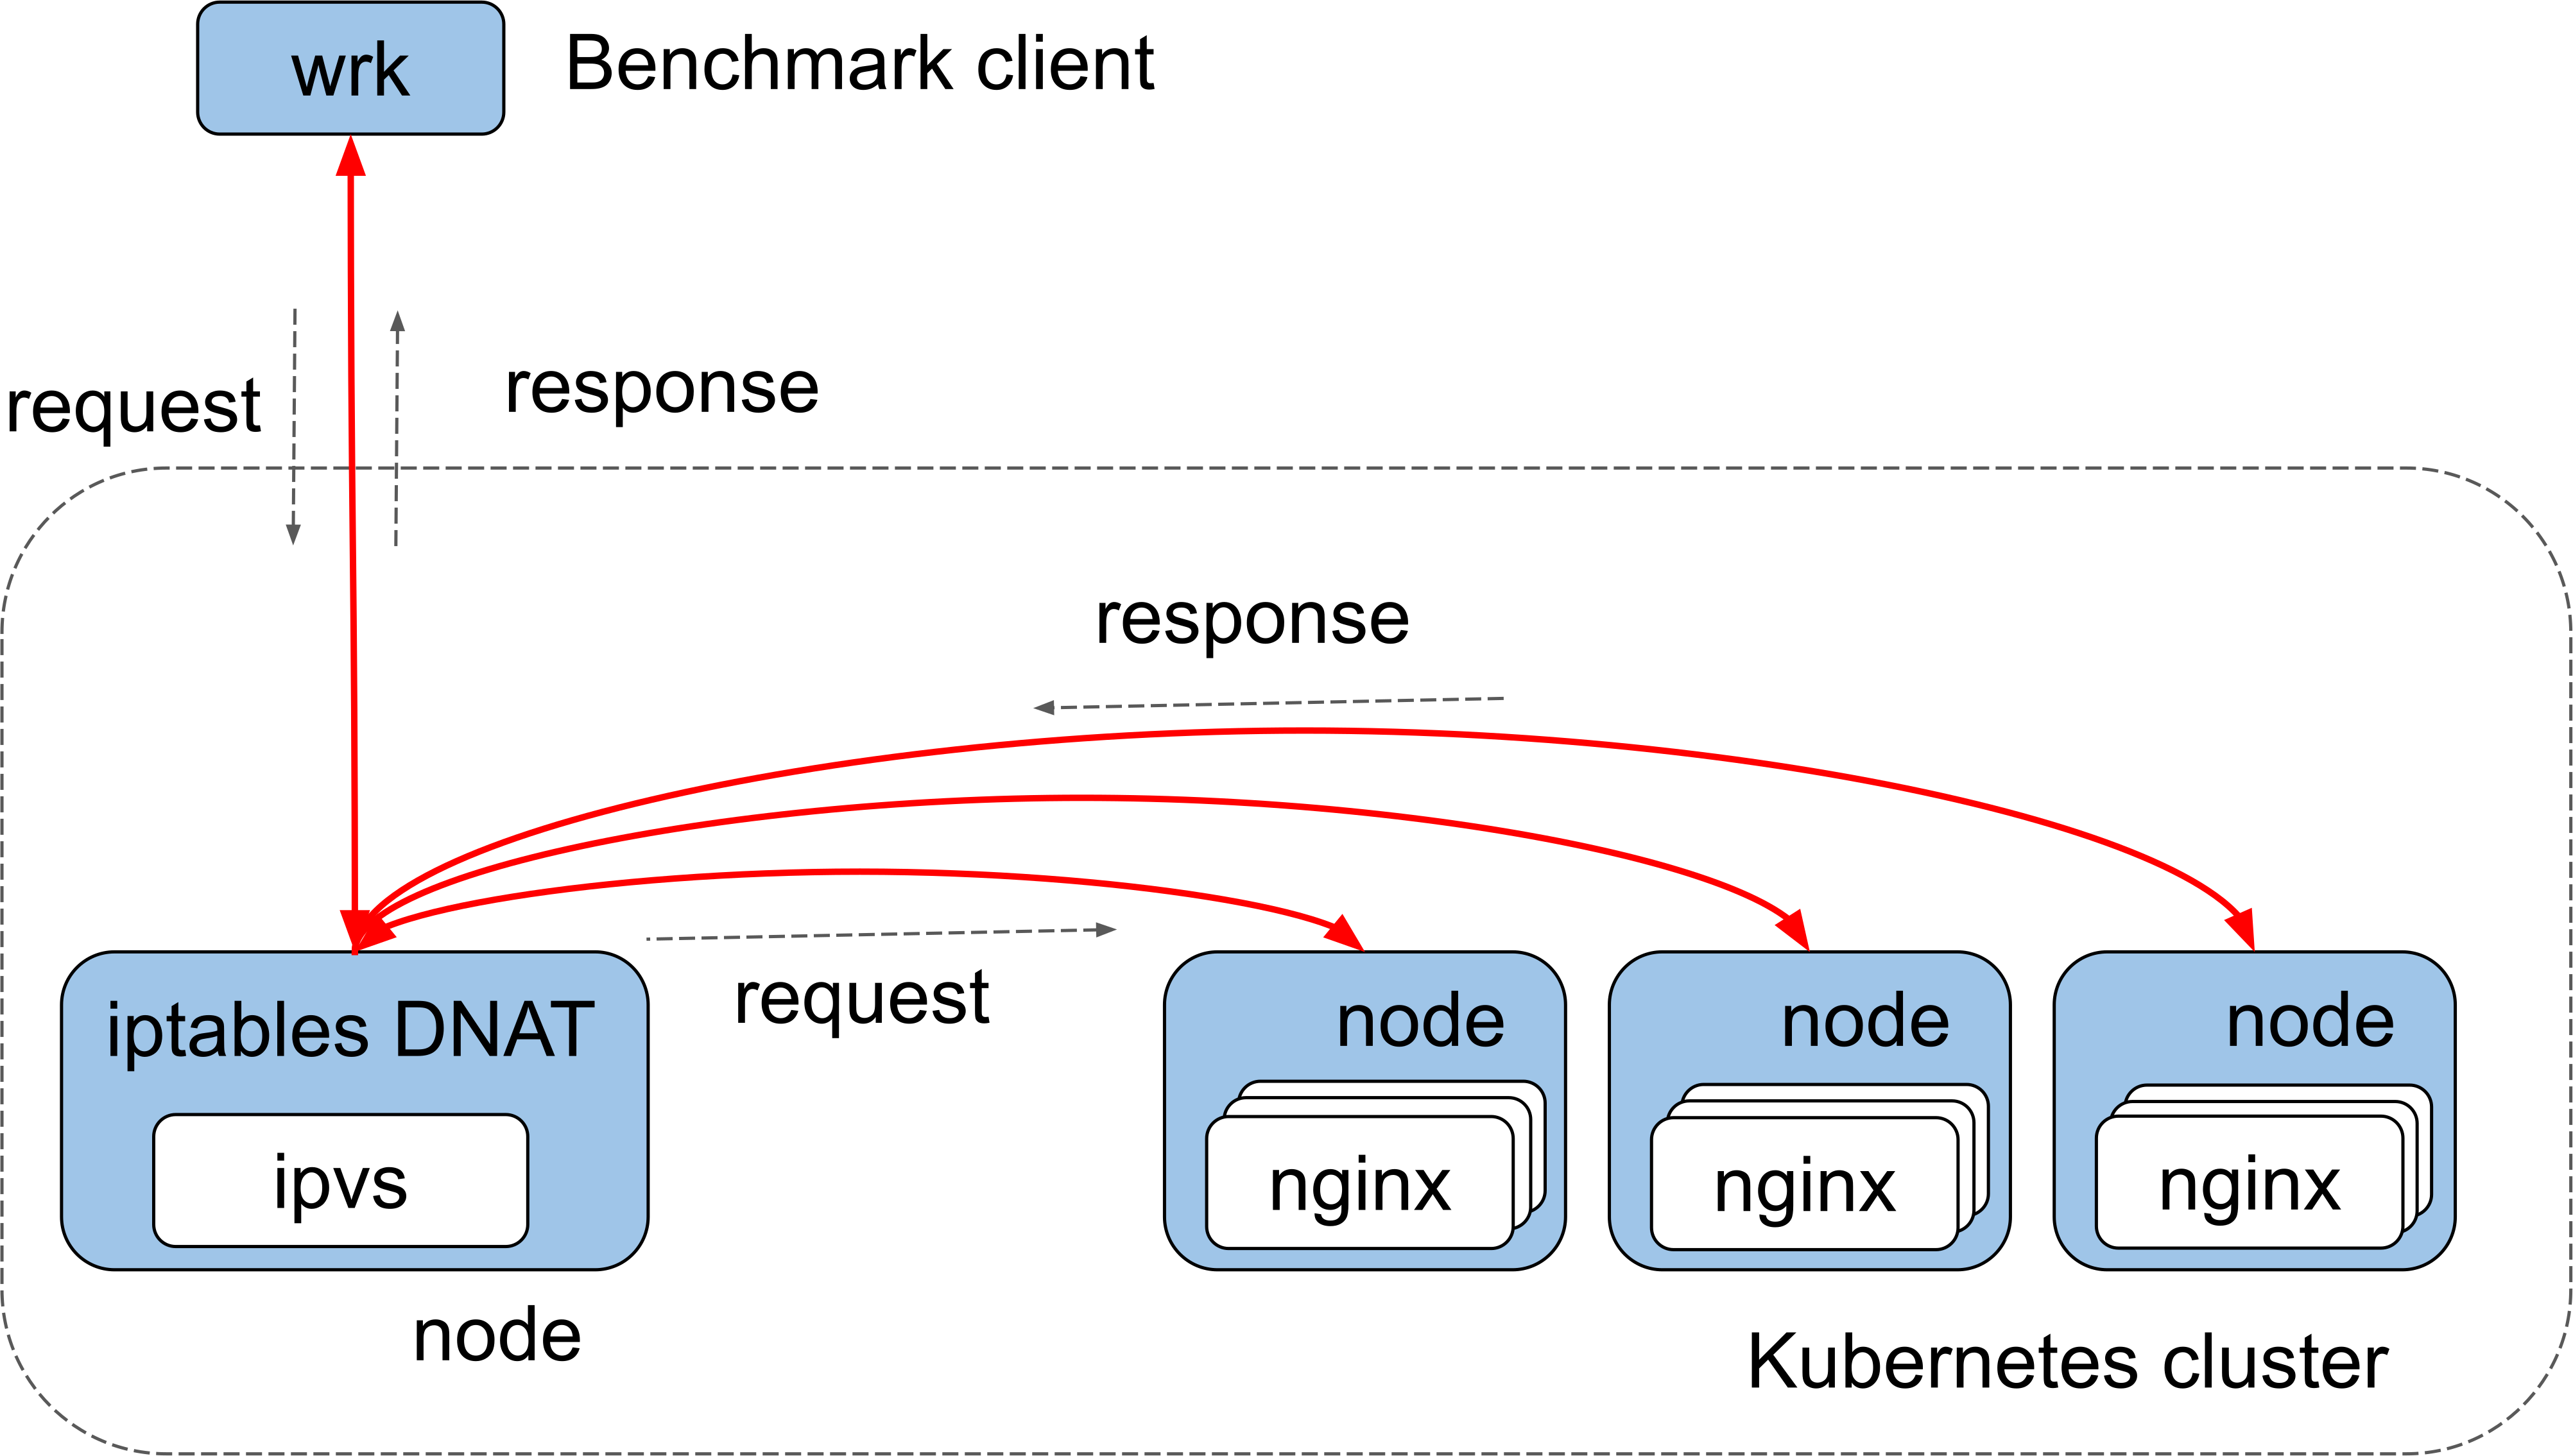
\includegraphics[width=0.8\columnwidth]{Figs/benchmark-schem-10g-nat}
    \par\bigskip
    \centering
    \begin{minipage}{0.9\columnwidth}
      \caption{}
      \label{fig:benchmark-schem-10g-nat}
    \end{minipage}
  \end{subfigure}

  \begin{subfigure}[t]{\columnwidth}
    \centering
    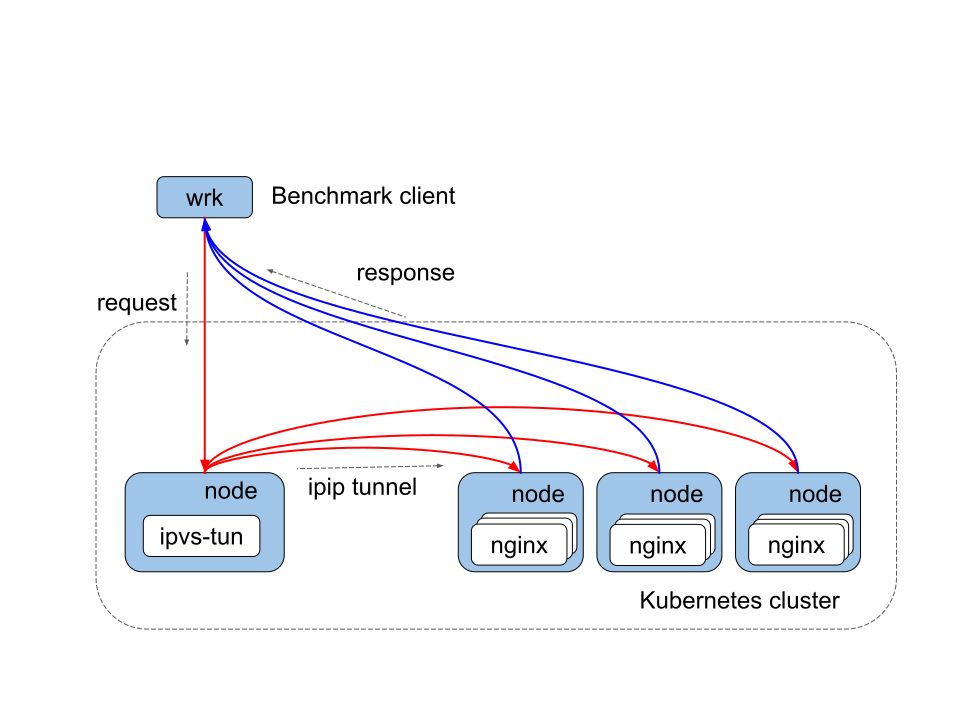
\includegraphics[width=0.8\columnwidth]{Figs/benchmark-schem-10g-dsr}
    \par\bigskip
    \centering
    \begin{minipage}{0.9\columnwidth}
      \caption{}
      \label{fig:benchmark-schem-10g-dsr}
    \end{minipage}
  \end{subfigure}

  \par\bigskip
  \centering
  \begin{minipage}{0.9\columnwidth}
    \caption[Benchmark setups in 10 Gbps experiment]{
      Benchmark setups in 10 Gbps experiment.
      (a) The setup used in throughput measurements of IPVS and iptables DNAT.
      The request and response packets both go through the load balancer node.
%      There is a bottleneck at the NIC of the load balancer node.
      (b) The setup used in throughput measurements of IPVS-TUN.
      The response packets for IPVS-TUN, return directly to the benchmark client.
%      The bottleneck is at the NIC of the benchmark client.
    }
    \label{fig:benchmark-schem-10g}
  \end{minipage}
\end{figure}

Figure~\ref{fig:benchmark-schem-10g} show experimental setups for the throughput measurements.
Multiple nginx {\em pods} are deployed on multiple nodes as web servers in the Kubernetes cluster.
In each nginx {\em pod}, single nginx web server program that returns the IP address of the {\em pod} itself is running.
The author then launched IPVS and IPVS-TUN pod as load balancers on one of the nodes, after that, the author performed the throughput measurement changing the number of the nginx web server pods.
On every Kubernetes node, there are iptables DNAT rules that function as an internal load balancer.
The author also measured throughput of the iptables DNAT as a load balancer.
The throughput is measured by sending out HTTP requests from the wrk towards a load balancer and by counting the number of responses the benchmark client received.
In the case of the IPVS-TUN, i.e., the tunneling mode of IPVS, the response packets follow the different route than the case of conventional IPVS and iptables DNAT.
As a result, the better performance level is expected for IPVS-TUN since the load balancer node only has to deal with request packets of the traffic.

\FloatBarrier

Figure~\ref{fig:ipvs_l3dsr_10g} shows the throughput results of IPVS, IPVS-TUN and iptables DNAT in 10 Gbps environment.
The general characteristics of a load balancer, where the throughput increases linearly to a saturation level as the number of nginx container increases, can be seen.
The maximum throughput of each load balancer is limited by either packet forwarding efficiency of the software load balancer itself or the bandwidth of the network.
The maximum throughput level of the iptables DNAT is close to 780k [req/sec], where the CPU usage of the benchmark client was 100\%.
The maximum throughput levels of IPVS and IPVS-TUN are less than that of iptables DNAT. 

\begin{figure}[h]
  \centering
  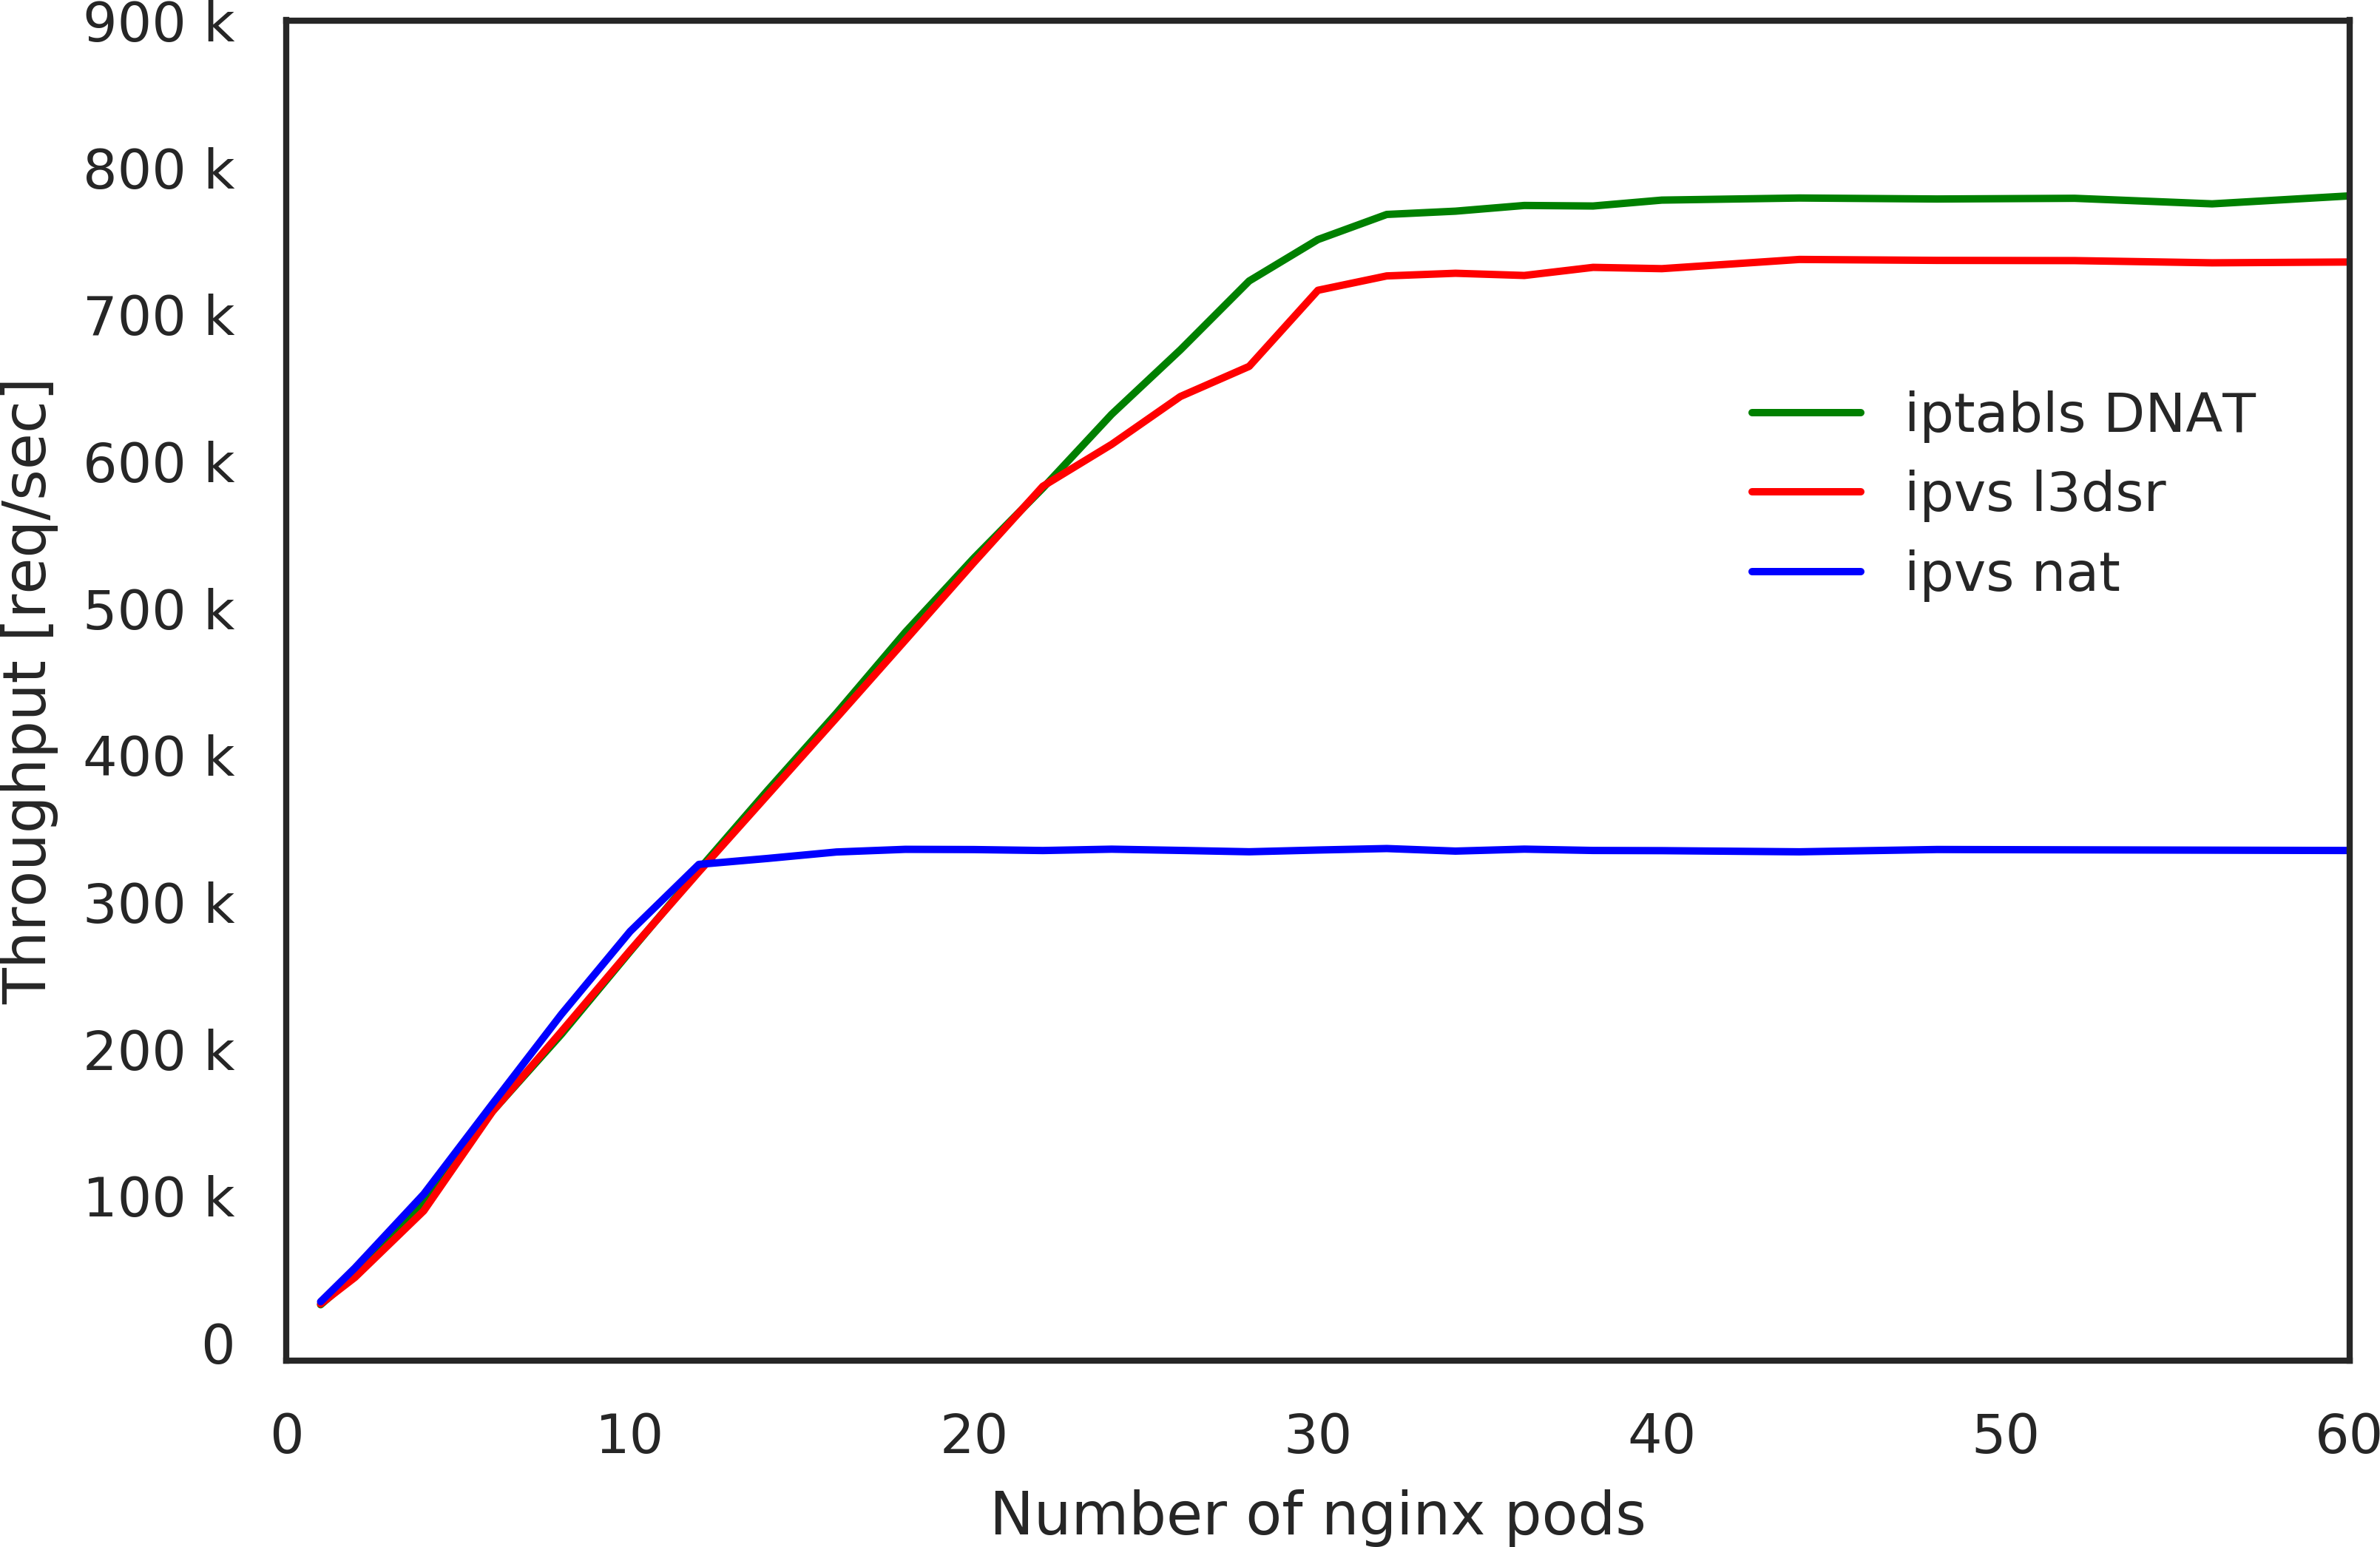
\includegraphics[width=0.8\columnwidth]{Figs/ipvs_l3dsr_10g}
  \par\bigskip
  \centering
  \begin{minipage}{0.9\columnwidth}
    \caption[Throughput of load balancers in 10 Gbps]{
      Throughput of load balancers in 10 Gbps.
      The iptables DNAT rules exist in the node net namespace.
      The IPVS and IPVS-TUN are in containers.
      The throughput of the iptables DNAT is the highest.
    }
    \label{fig:ipvs_l3dsr_10g}
  \end{minipage}
\end{figure}

Figure~\ref{fig:ipvs_l3dsr_10g} shows comparison of CPU usage between load balancers.
CPU usages are sampled on the load balancer nodes at the time of the throughput measurement using a program called dstat \cite{wieers2019dstat}.
It is seen that IPVS-TUN uses less CPU resource than IPVS because the load balancer node does not have to deal with the response packets.
The iptables DNAT uses even less CPU resource than IPVS and IPVS-TUN.
Possible reasons for the lesser performance levels for IPVS are as follows;
(1) It is possible that the IPVS and IPVS-TUN program themselves are less efficient than iptables DNAT.
(2) The network setup for the container, i.e., bridge+veth may be causing the overhead.
While iptables DNAT rules exist in node net namespace, proposed IPVS and IPVS-TUN exist in container net namespace.
In order to clarify which of these is the true reason for the performance difference, the author carried out throughput measurement for IPVS and IPVS-TUN without using the container network, i.e., in node net namespaces.

\begin{figure}[h]
  \centering
  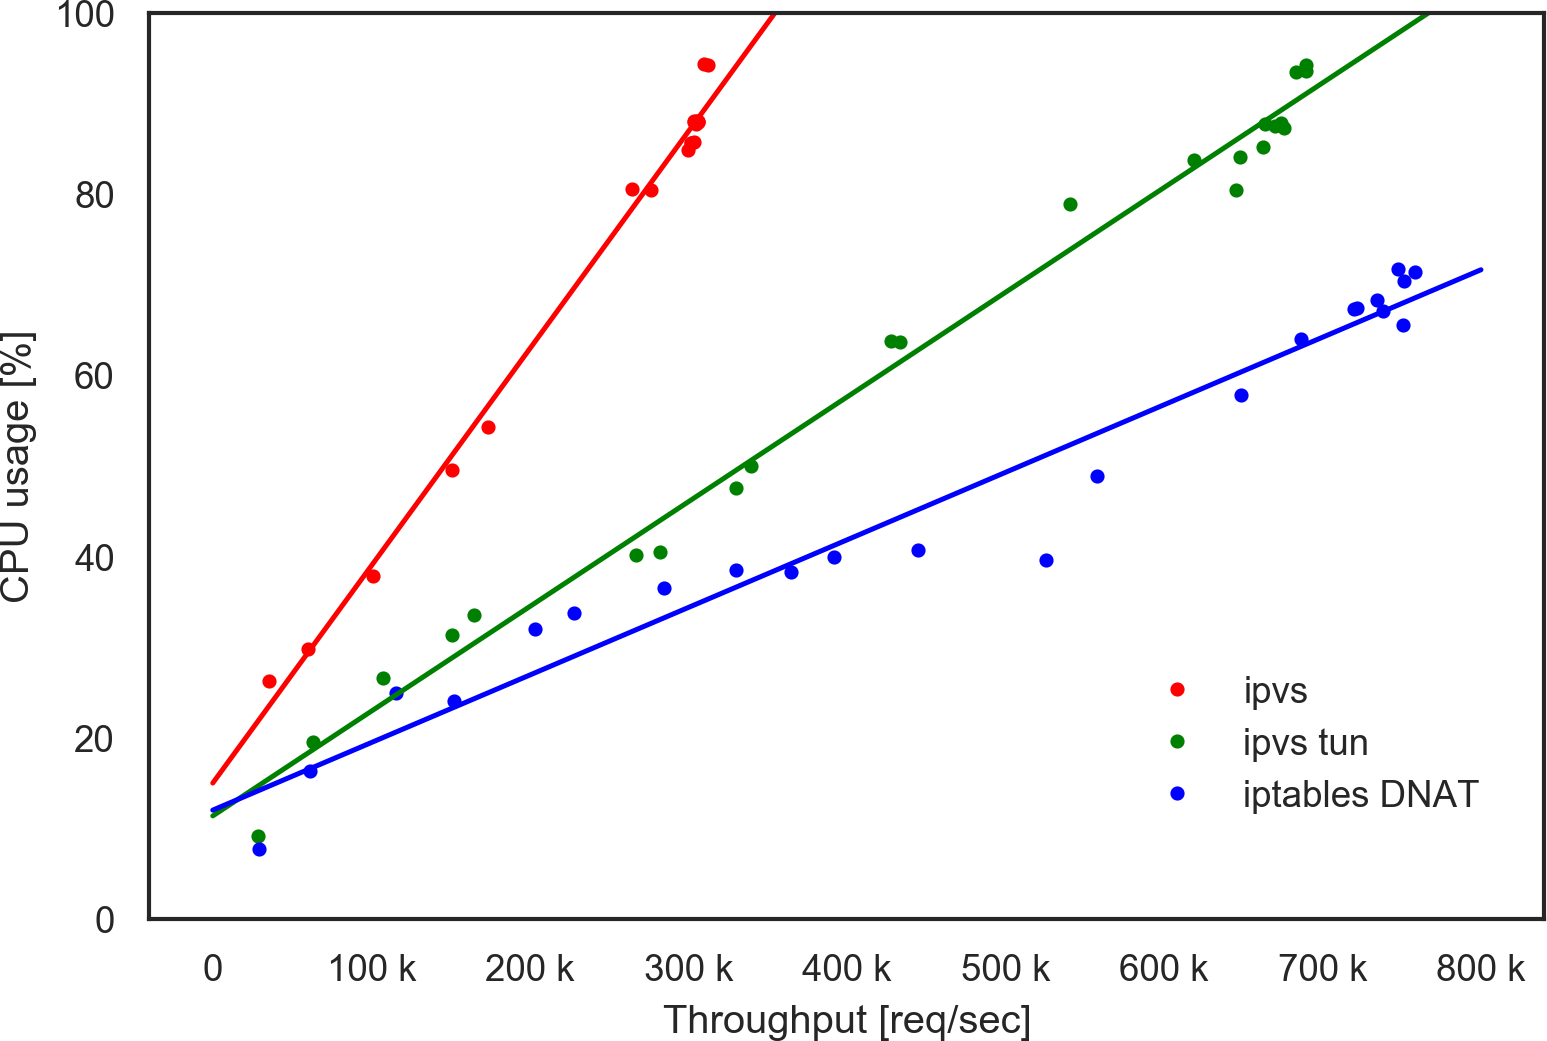
\includegraphics[width=0.8\columnwidth]{Figs/cpu_usage_10g}
  \par\bigskip
  \centering
  \begin{minipage}{0.9\columnwidth}
    \caption[CPU usage of load balancers in containers]{
      CPU usage of load balancers in containers.
      The iptables DNAT rules exist in the node net namespace.
      The IPVS and IPVS-TUN are in containers.
      The iptables DNAT consumes the smallest amount of the CPU resource.
    }
    \label{fig:cpu_usage_10g}
  \end{minipage}
\end{figure}

\FloatBarrier

\subsubsection{Performance comparison in node net namespace}

The IPVS and IPVS-TUN load balancers were setup on one of the nodes. 
The load balancing rules were created in the node namespaces, and then throughput measurement were carried out.

Figure~\ref{fig:ipvs_l3dsr_10g_node_ns} shows the throughput of IPVS and IPVS-TUN in the node net namespace together with the throughput of the iptables DNAT.
The throughputs of the IPVS and IPVS-TUN are improved from the previous results in Figure~\ref{fig:ipvs_l3dsr_10g}.
This improvement indicates that the overhead due to container network using veth+bridge has a significant impact.
%
The throughput of the IPVS-TUN is almost identical to that of iptables DNAT.
The maximum throughput of these are probably limited by the performance of the benchmark client since the CPU usages of the benchmark client at the saturation level were almost 100\% in both cases.

\begin{figure}[h]
  \centering
  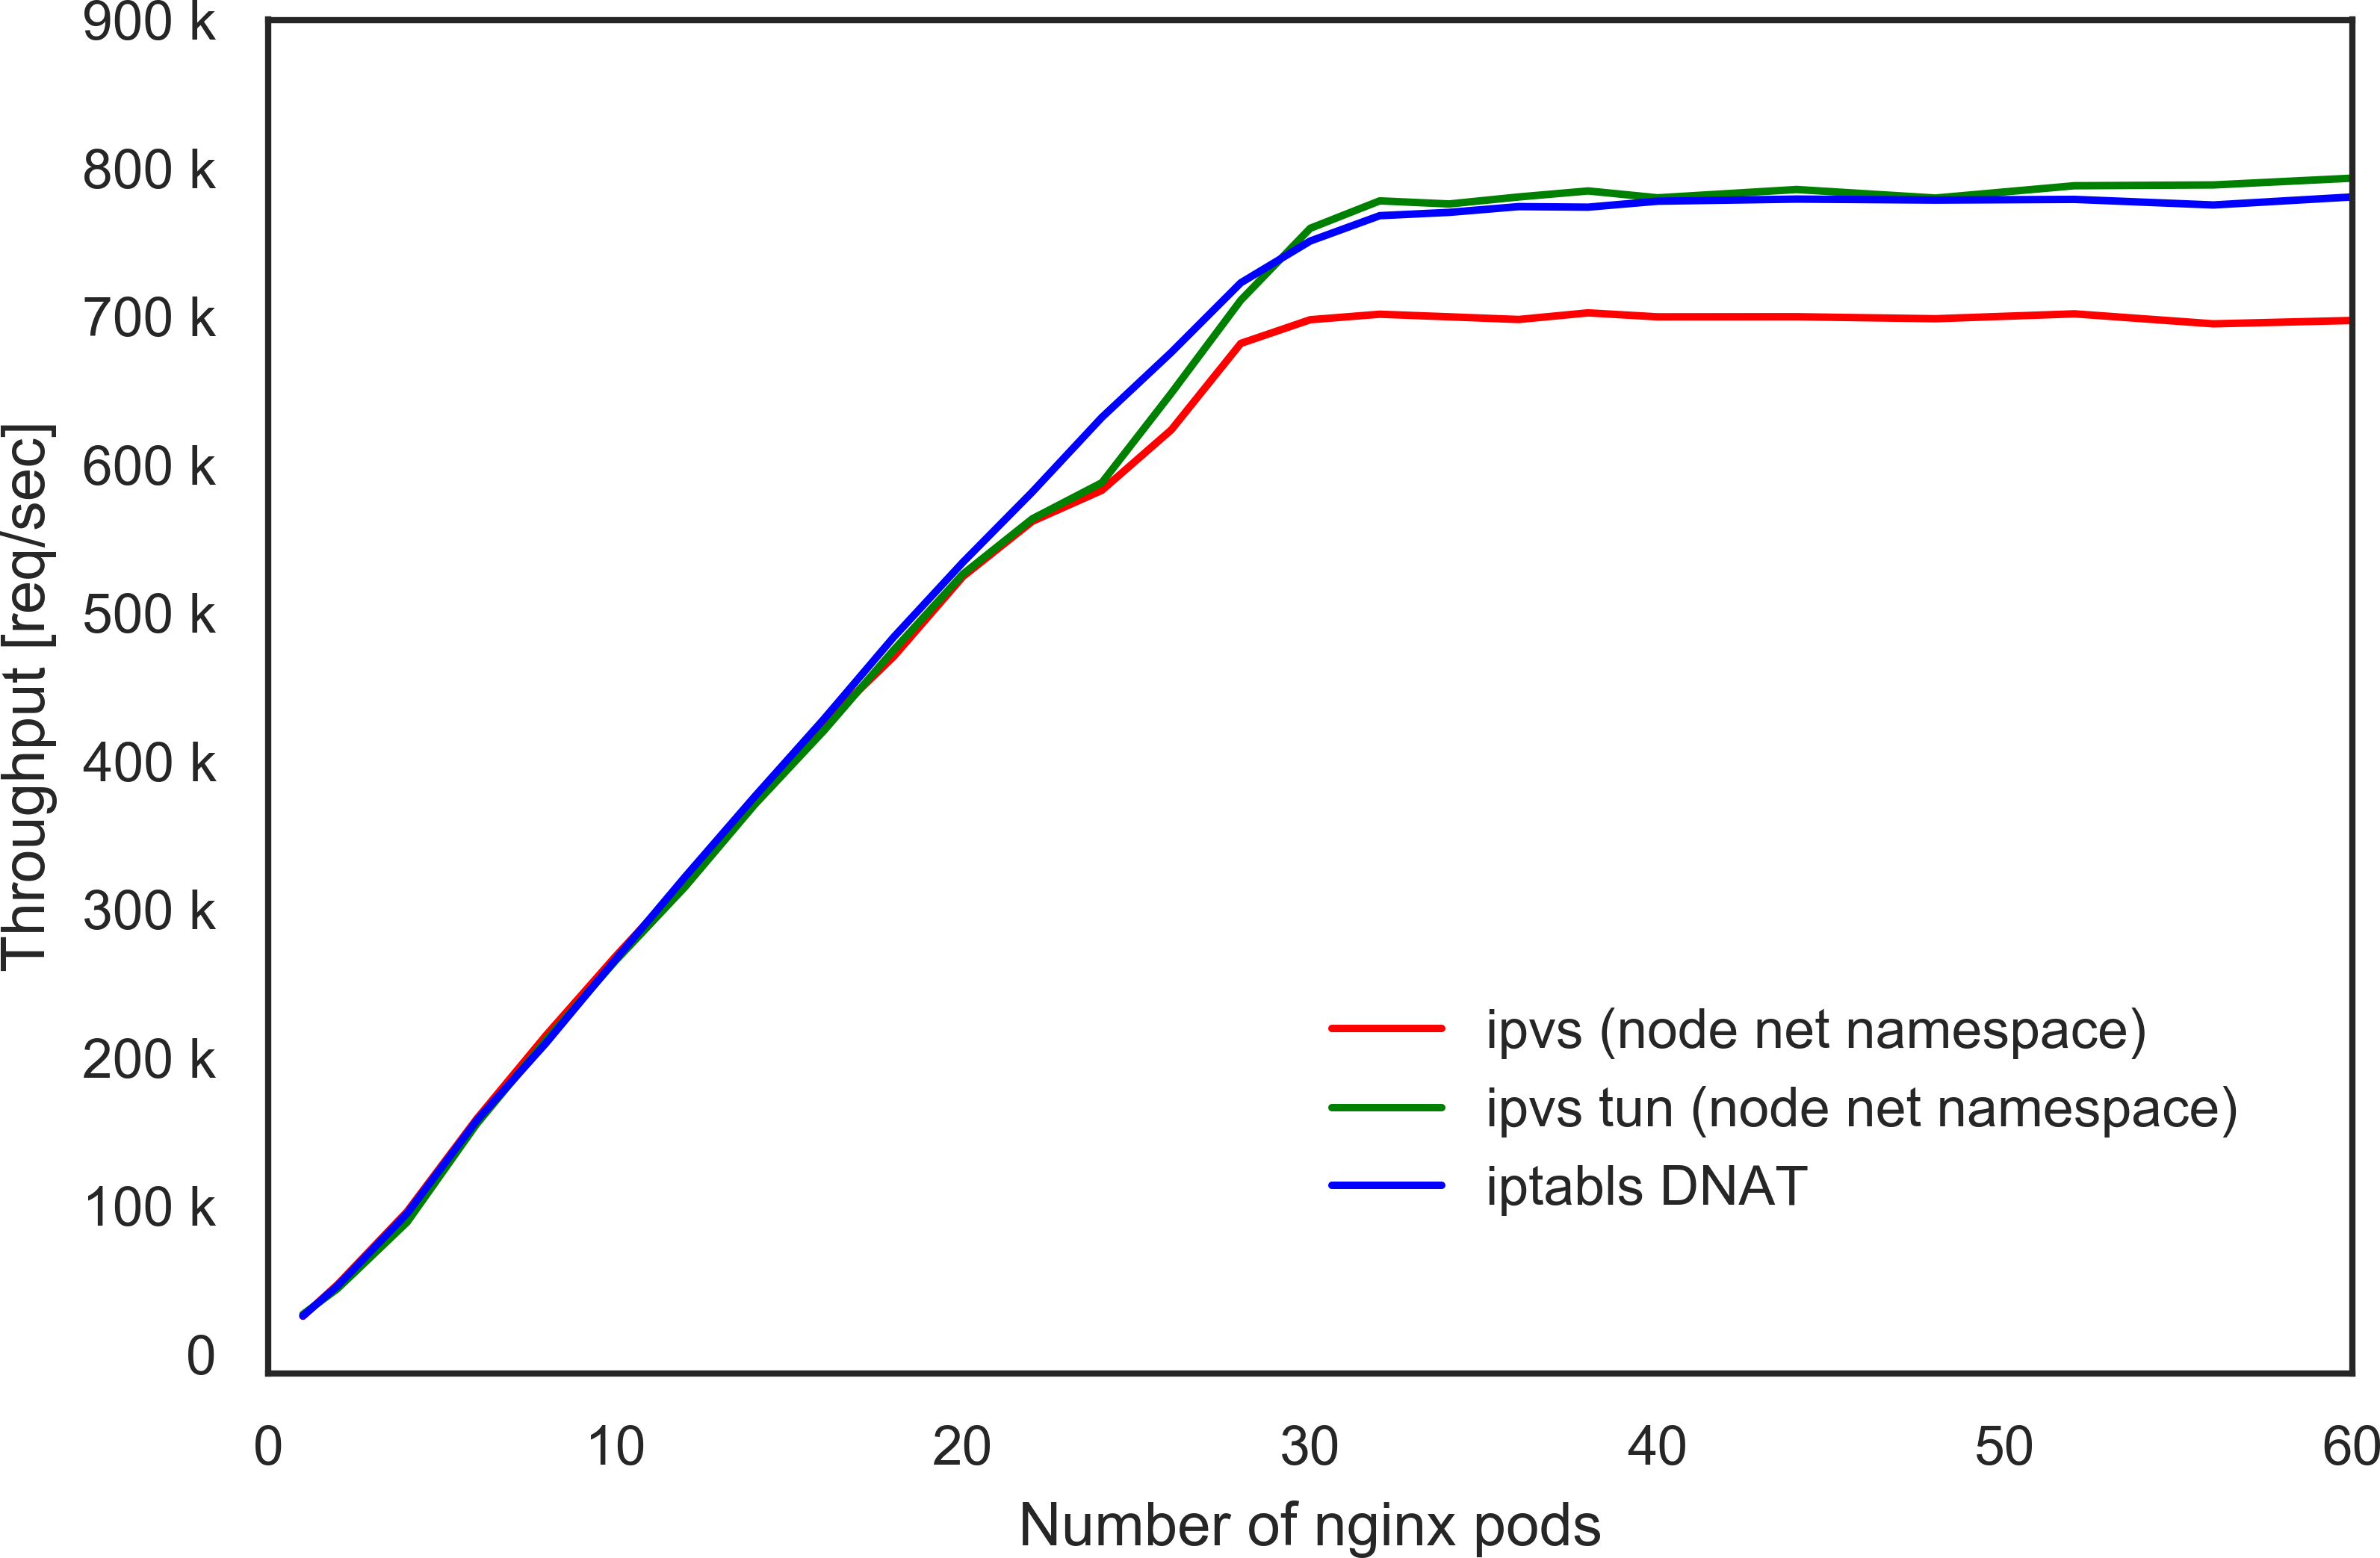
\includegraphics[width=0.8\columnwidth]{Figs/ipvs_l3dsr_10g_node_ns}
  \par\bigskip
  \centering
  \begin{minipage}{0.9\columnwidth}
    \caption[Throughput of load balancers in node namespace]{
      Throughput of load balancers in node namespace.
      The performance levels of the IPVS and IPVS-TUN are greatly improved from those in Figure~\ref{fig:ipvs_l3dsr_10g} by placing them in node net namespace.
    }
    \label{fig:ipvs_l3dsr_10g_node_ns}
  \end{minipage}
\end{figure}

Figure~\ref{fig:cpu_usage_10g_node_ns} shows CPU usages of each load balancers.
The CPU usage of the IPVS-TUN is smaller than that of IPVS.
This is because the load balancer does not process the response packets in L3DSR setting.
The CPU usage of the IPVS is still more extensive than that of iptables DNAT, indicating that IPVS is inherently less efficient than iptables DNAT.

\begin{figure}[h]
  \centering
  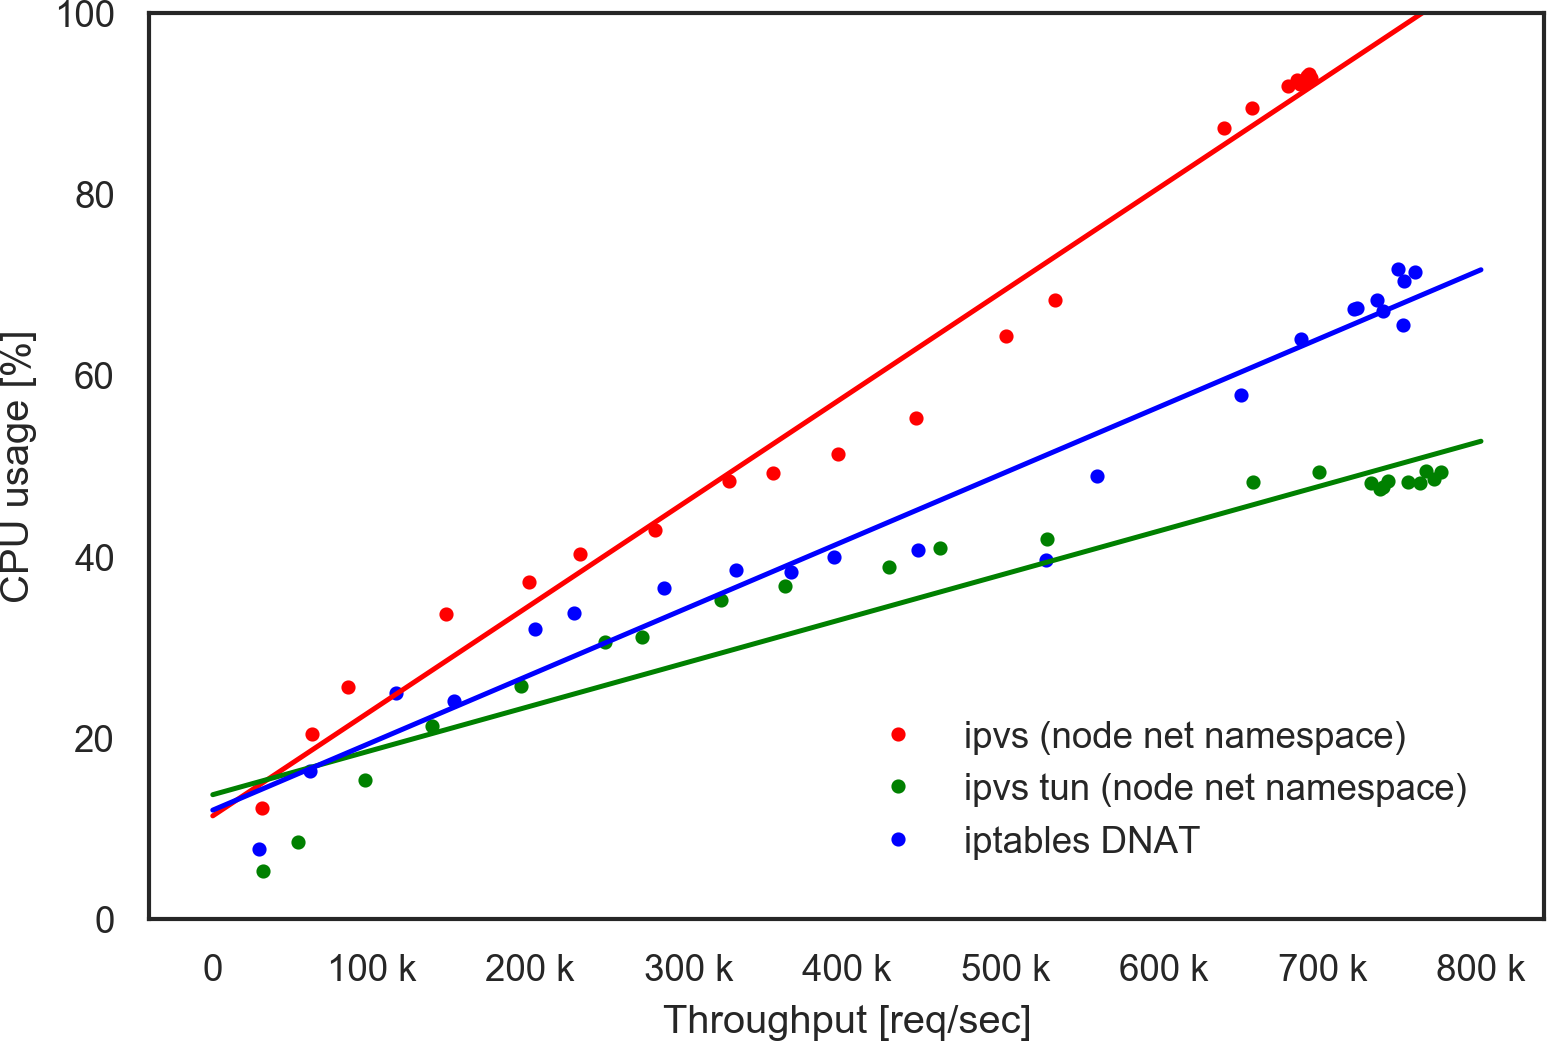
\includegraphics[width=0.8\columnwidth]{Figs/cpu_usage_10g_node_ns}
  \par\bigskip
  \centering
  \begin{minipage}{0.9\columnwidth}
    \caption[CPU usage of load balancers on nodes]{
      CPU usage of load balancers on nodes.
      CPU usages of IPVS and IPVS-TUN greatly improved from those in Figure~\ref{fig:cpu_usage_10g} by placing them in node net namespace.  
      While the IPVS-TUN consumes the smallest amount of the CPU resource, the CPU usage of IPVS is still larger than that of iptables DNAT.
    }
    \label{fig:cpu_usage_10g_node_ns}
  \end{minipage}
\end{figure}

The author summarizes this section as follows;
The IPVS itself is less efficient than iptables DNAT.
Using the container network, i.e., veth+bridge further degrades the throughput of IPVS.
Therefore, both of these are the reasons for inferior performance levels for IPVS and IPVS-TUN in containers.

\FloatBarrier

\section{Discussion of required throughput}

The author has compared the performance of proposed load balancers in 10 Gbps in the previous section.
Although the proposed load balancer may not be the most efficient one, herein, the author shows that it has sufficient throughput for 10 Gbps network environment.

Table~\ref{tab:performance_summary} summarizes the maximum throughputs of the different load balancers obtained in the experiments so far.
Depending on the experimental conditions different part of the experimental setup limits the throughput of the load balancers.
Since the performance bottlenecks are mainly due to network bandwidth in 1 Gbps network, it is easy to estimate the possible bottleneck due to bandwidth in a faster network.
Since benchmark client exists at the location where normally the upstream router exists, the performance bottleneck at the benchmark client corresponds to the maximum throughput that the load balancer should handle.

\begin{table}[H]

  \begin{subtable}{1\textwidth}
    \centering
    \begin{tabular}{|l|l|c|l|}
      \hline
      \multicolumn{1}{|c|}{Type} & \multicolumn{1}{c|}{namespace} &
      \begin{tabular}{c} Throughput \\ {[}req/sec{]} \end{tabular} & \multicolumn{1}{c|}{Bottleneck} \\ \hline
      iptables DNAT & node      & 193K &
      \begin{tabular}{l} Bandwidth filled with request \\ + response @ load balancer \end{tabular} \\ \hline
      IPVS          & container & 197K &
      \begin{tabular}{l} Bandwidth filled with request \\ + response @ load balancer \end{tabular} \\ \hline
      IPVS-TUN      & container & 293K &
      \begin{tabular}{l} Bandwidth filled with response \\ @ benchmark client  \end{tabular} \\ \hline
    \end{tabular}
    \caption{1 Gbps experiment}
  \end{subtable}

  \par\bigskip

  \begin{subtable}{1\textwidth}
    \centering
    \begin{tabular}{|l|l|c|l|}
      \hline
      \multicolumn{1}{|c|}{Type} & \multicolumn{1}{c|}{namespace} &
      \begin{tabular}{c} Throughput \\ {[}req/sec{]} \end{tabular} & \multicolumn{1}{c|}{Bottleneck} \\ \hline
      iptables DNAT & node      & 778K & \begin{tabular}{l} CPU\(\sim\)100\% @ benchmark client\end{tabular} \\ \hline
      IPVS          & container & 335K & \begin{tabular}{l} CPU\(\sim\)100\% @ load balancer node\end{tabular} \\ \hline
      IPVS-TUN      & container & 731K & \begin{tabular}{l} CPU\(\sim\)100\% @ load balancer node\end{tabular} \\ \hline
      IPVS          & node      & 700K & \begin{tabular}{l} CPU\(\sim\)100\% @ load balancer node\end{tabular} \\ \hline
      IPVS-TUN      & node      & 780K & \begin{tabular}{l} CPU\(\sim\)100\% @ benchmark client\end{tabular} \\ \hline
   \end{tabular}
      \caption{10 Gbps experiment}
  \end{subtable}

  \par\bigskip
  \centering
  \begin{minipage}{0.9\columnwidth}
    \caption[Summary of the maximum throughputs]{
      Summary of the maximum throughputs.
    }
    \label{tab:performance_summary}
  \end{minipage}
\end{table}
    
For example, the bottleneck at the benchmark client is about 293K [req/sec] in the 1 Gbps network. 
The load balancers only need to be able to handle at most 293K [req/sec] equivalent of the traffic.
Even if the load balancer is capable of handling 500K [req/sec], the throughput of the system is ultimately determined by the bottleneck at the entrance, that is 293K [req/sec].
The maximum throughput in 1 Gbps, i.e., 293K [req/seq] is already achieved by single IPVS-TUN (293K [req/seq]) or two of IPVS load balancers (193K x 2 [req/seq]) with ECMP redundancy.

In the case of 10 Gbps network, the maximum throughput determined by the bottleneck at the entrance \replaced[id=5th]{becomes}{is} 2.9M [req/sec].
Single IPVS-TUN cannnot handle this much of the traffic.
However, this is still  achievable without much of the hassle by using four of IPVS-TUN (731K x 4 [req/seq]) or nine of IPVS load balancers (335K x 9 [req/seq]) with ECMP redundancy.

In the case of 100 Gbps network, where the load balancers are required to handle up to 29M [req/sec] of the throughput, the inefficiency of the software load balancer in a container can become a real problem.
Because in order to handle 29M [req/sec] of the traffic, 90 of IPVS load balancer would be needed.
In this case, more efficient load balancer or container network is needed.
In the next section, the author tries to improve the efficiency of a load balancer, by implementing novel XDP load balancer.
Except for such cases, the proposed load balancer can provide sufficient throughput.

\FloatBarrier

\section{XDP load balancer}

The eXpress Data Path (XDP) \cite{hoiland2018express} is Linux kernel technology recently developed, where the tools and functionality to intercept and process the packets in the earliest phase as possible are provided.
By using XDP, one can write packet manipulation code using a subset of the C programing language, byte-compile it, and hook it into the place before the socket buffer is assigned, thereby speeding up network manipulation.
Typical applications include packet drop against DDOS attack, simple packet forwarding, and load balancing.
One of the benefits of the XDP compared to the technology using Data Plane Development Kit (DPDK) \cite{dpdkorg} is that in the case of XDP, the packets that do not match the rule for processing are then passed to normal Linux kernel's network stack.
Therefore there is no need for preparing dedicated NIC for fast and efficient network processing.
The author implemented the XDP load balancer and carried out throughput measurement.

\subsubsection{Implementation}

Figure~\ref{fig:xlb-schem} show schematic diagram of the XDP load balancer, xlb, which is implemented by the author.
The xlb consists of programs and configurations shown in Table~\ref{table:xlb-progs}.
The xlb\_kernel.ll is the byte-compiled eBPF program that actually process the packets based on the load balance rules in the xlb table.
Load balancing rules are populated by a userspace daemon xlbd from the configration file xlbd.conf and nexthop and MAC address information obtained from the Linux kernel.

\begin{figure}[h]
  \centering
  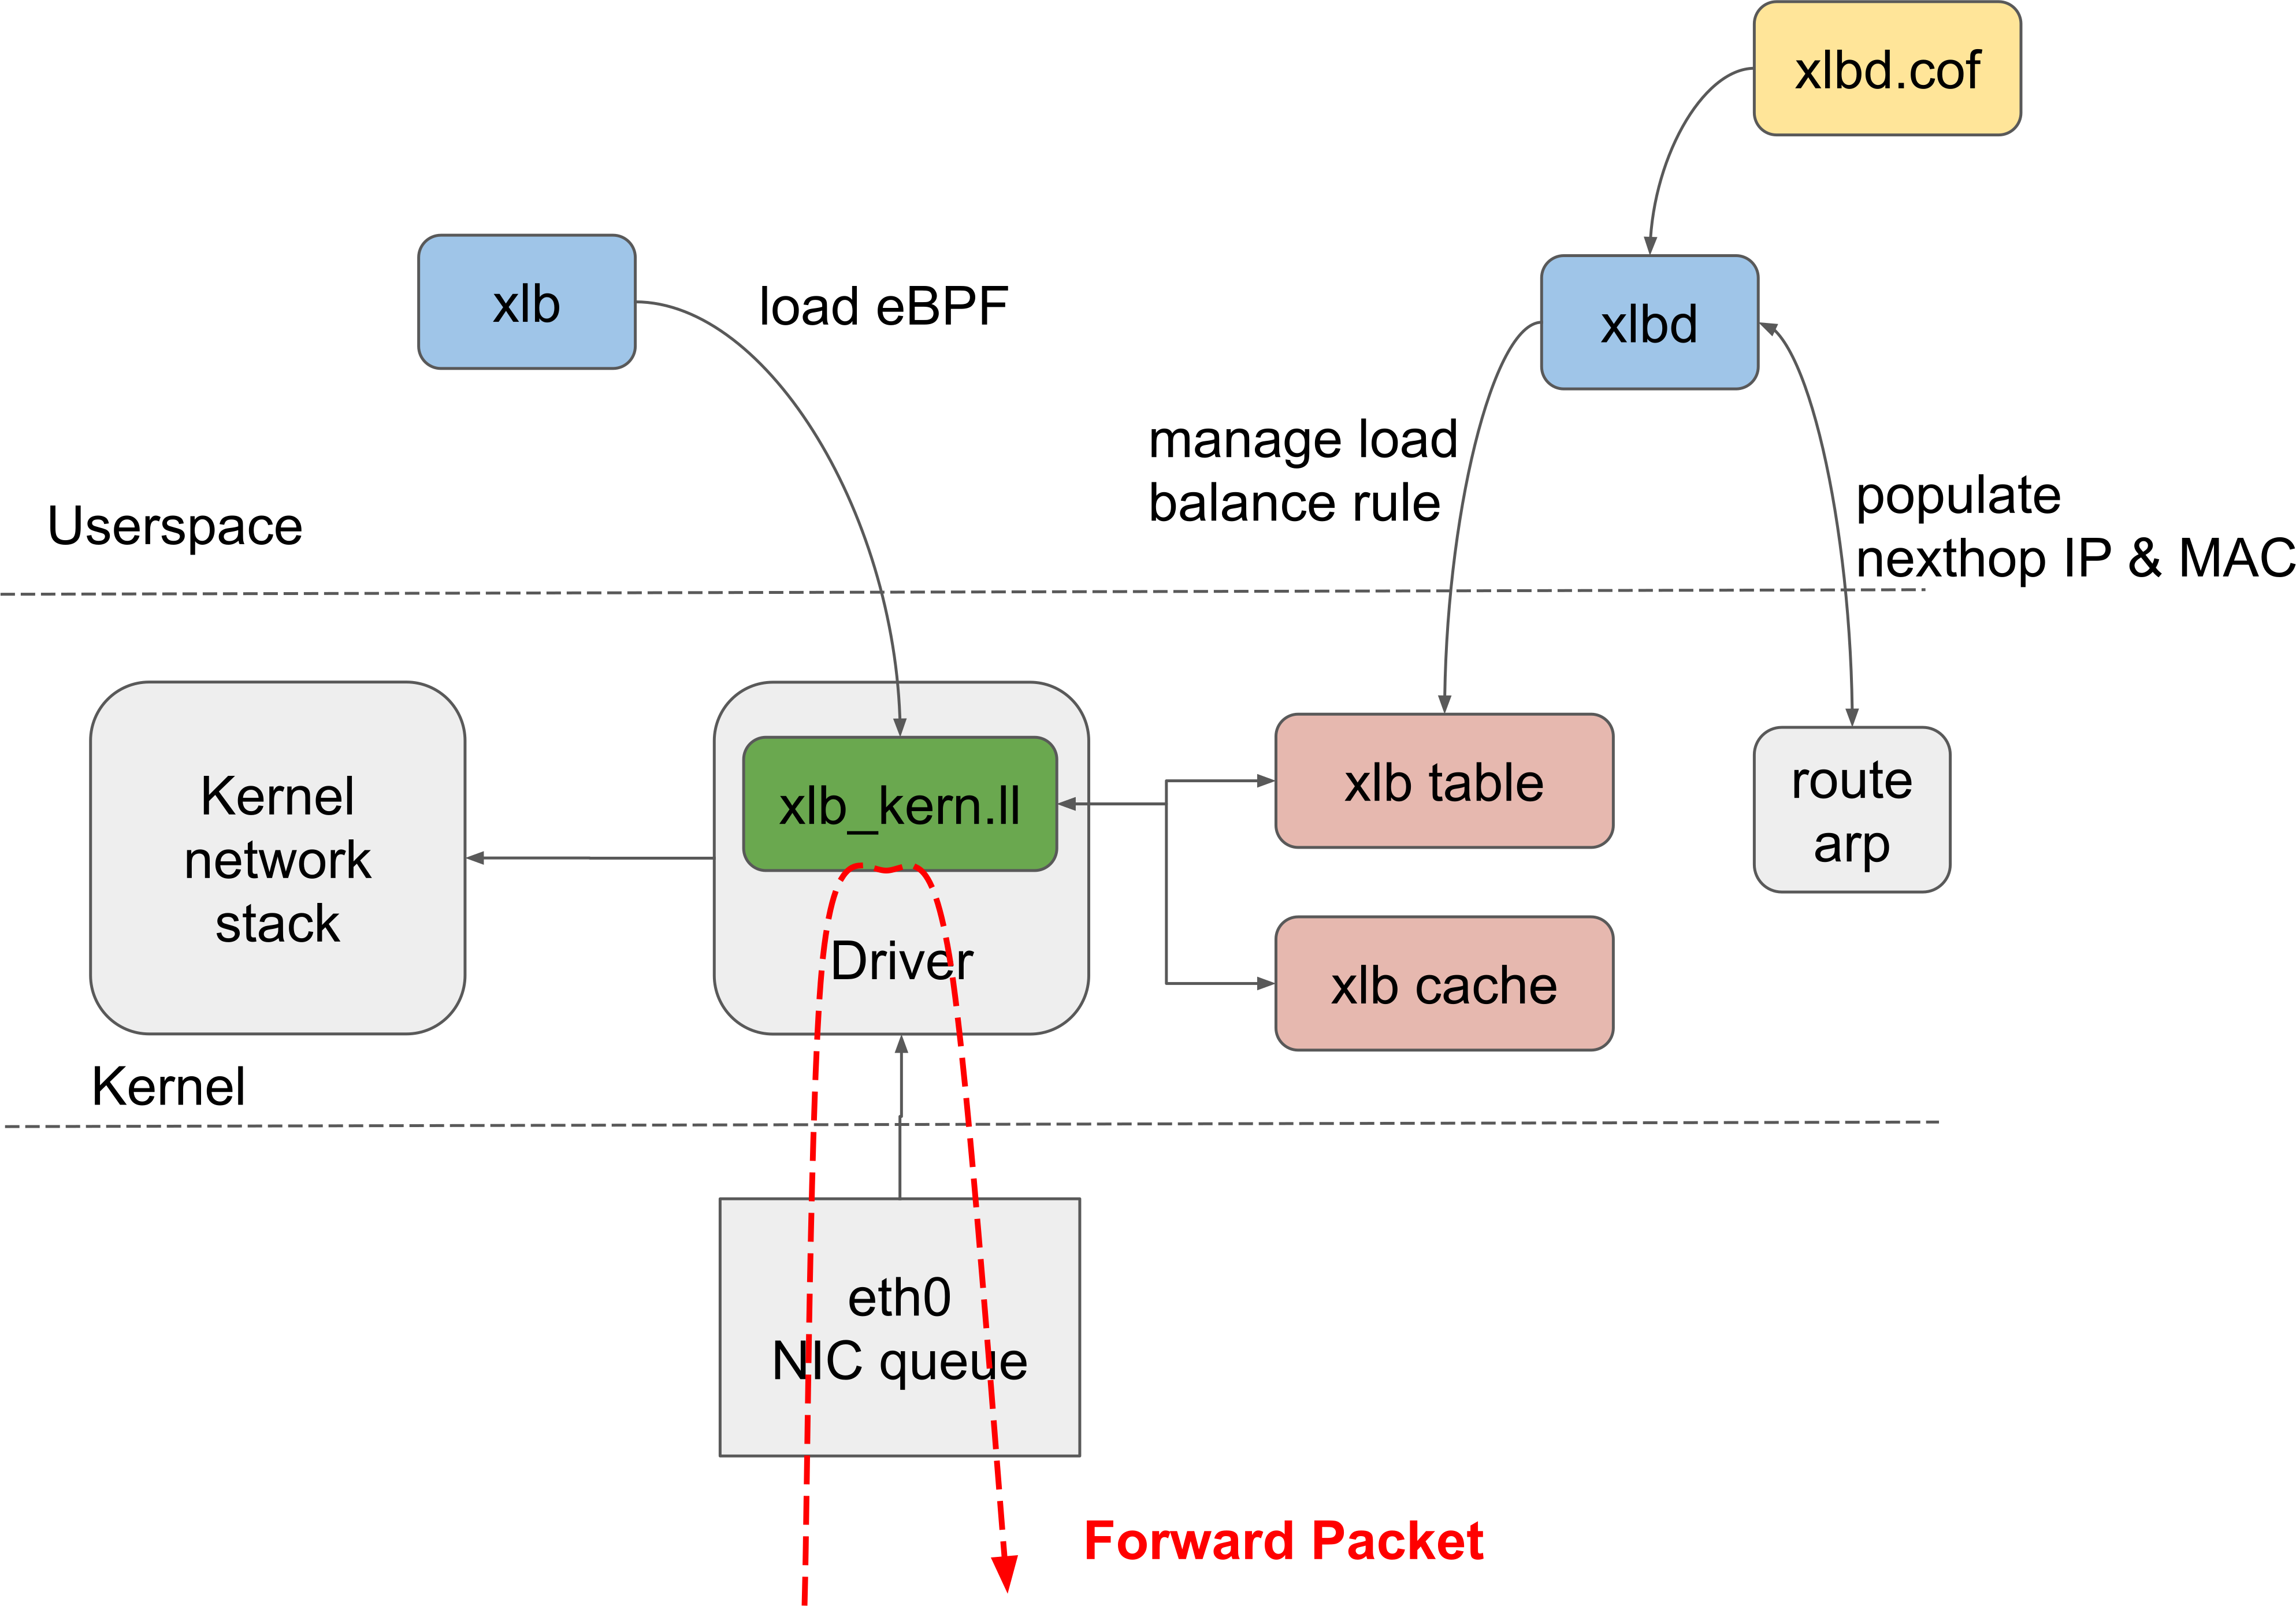
\includegraphics[width=0.9\columnwidth]{Figs/xlb-schem}

  \par\bigskip
  \centering
  \begin{minipage}{0.9\columnwidth}
    \caption[Xlb architecture]{
      Xlb architecture.
      The author implemented an XDP load balancer named xlb.
    }
    \label{fig:xlb-schem}
  \end{minipage}
\end{figure}

\begin{table}[h]
  \centering
  \begin{tabular}{|l|l|}
    \hline
    Name & Function \\ \hline
    xlb\_kern.ll & byte compiled eBPF program  \\ \hline
    xlb & utility to inject eBPF program into kernl  \\ \hline
    xlbd & daemon to control load balance table  \\ \hline
    xlbd.conf & load balancing configuration  \\ \hline
    xlb table & load balance table  \\ \hline
    xlb cache & load balance cache  \\ \hline
  \end{tabular}

  \par\bigskip
  \centering
  \begin{minipage}{0.9\columnwidth}
    \caption[Xlb components]{
      Xlb components.
    }
    \label{table:xlb-progs}
  \end{minipage}
\end{table}

%% \subsubsection{Benchmark setup}

\subsubsection{Throughput results }

The author carried out the throughput measurement for the XDP load balancer, xlb.
The hardware and software configurations are same as the ones in Table~\ref{tab:hw_sw_spec_10g}.
The experimental setup is also same as the one in Figure~\ref{fig:benchmark-schem-10g}(b).
Since current implementation of xlb does not support multi core packet processing, the setting \enquote{(RSS,RPS)=(off,off)} is used in the throughput measurement.
All the interrupt from the NIC are notified to a single core.

\begin{figure}[h]
  \centering
  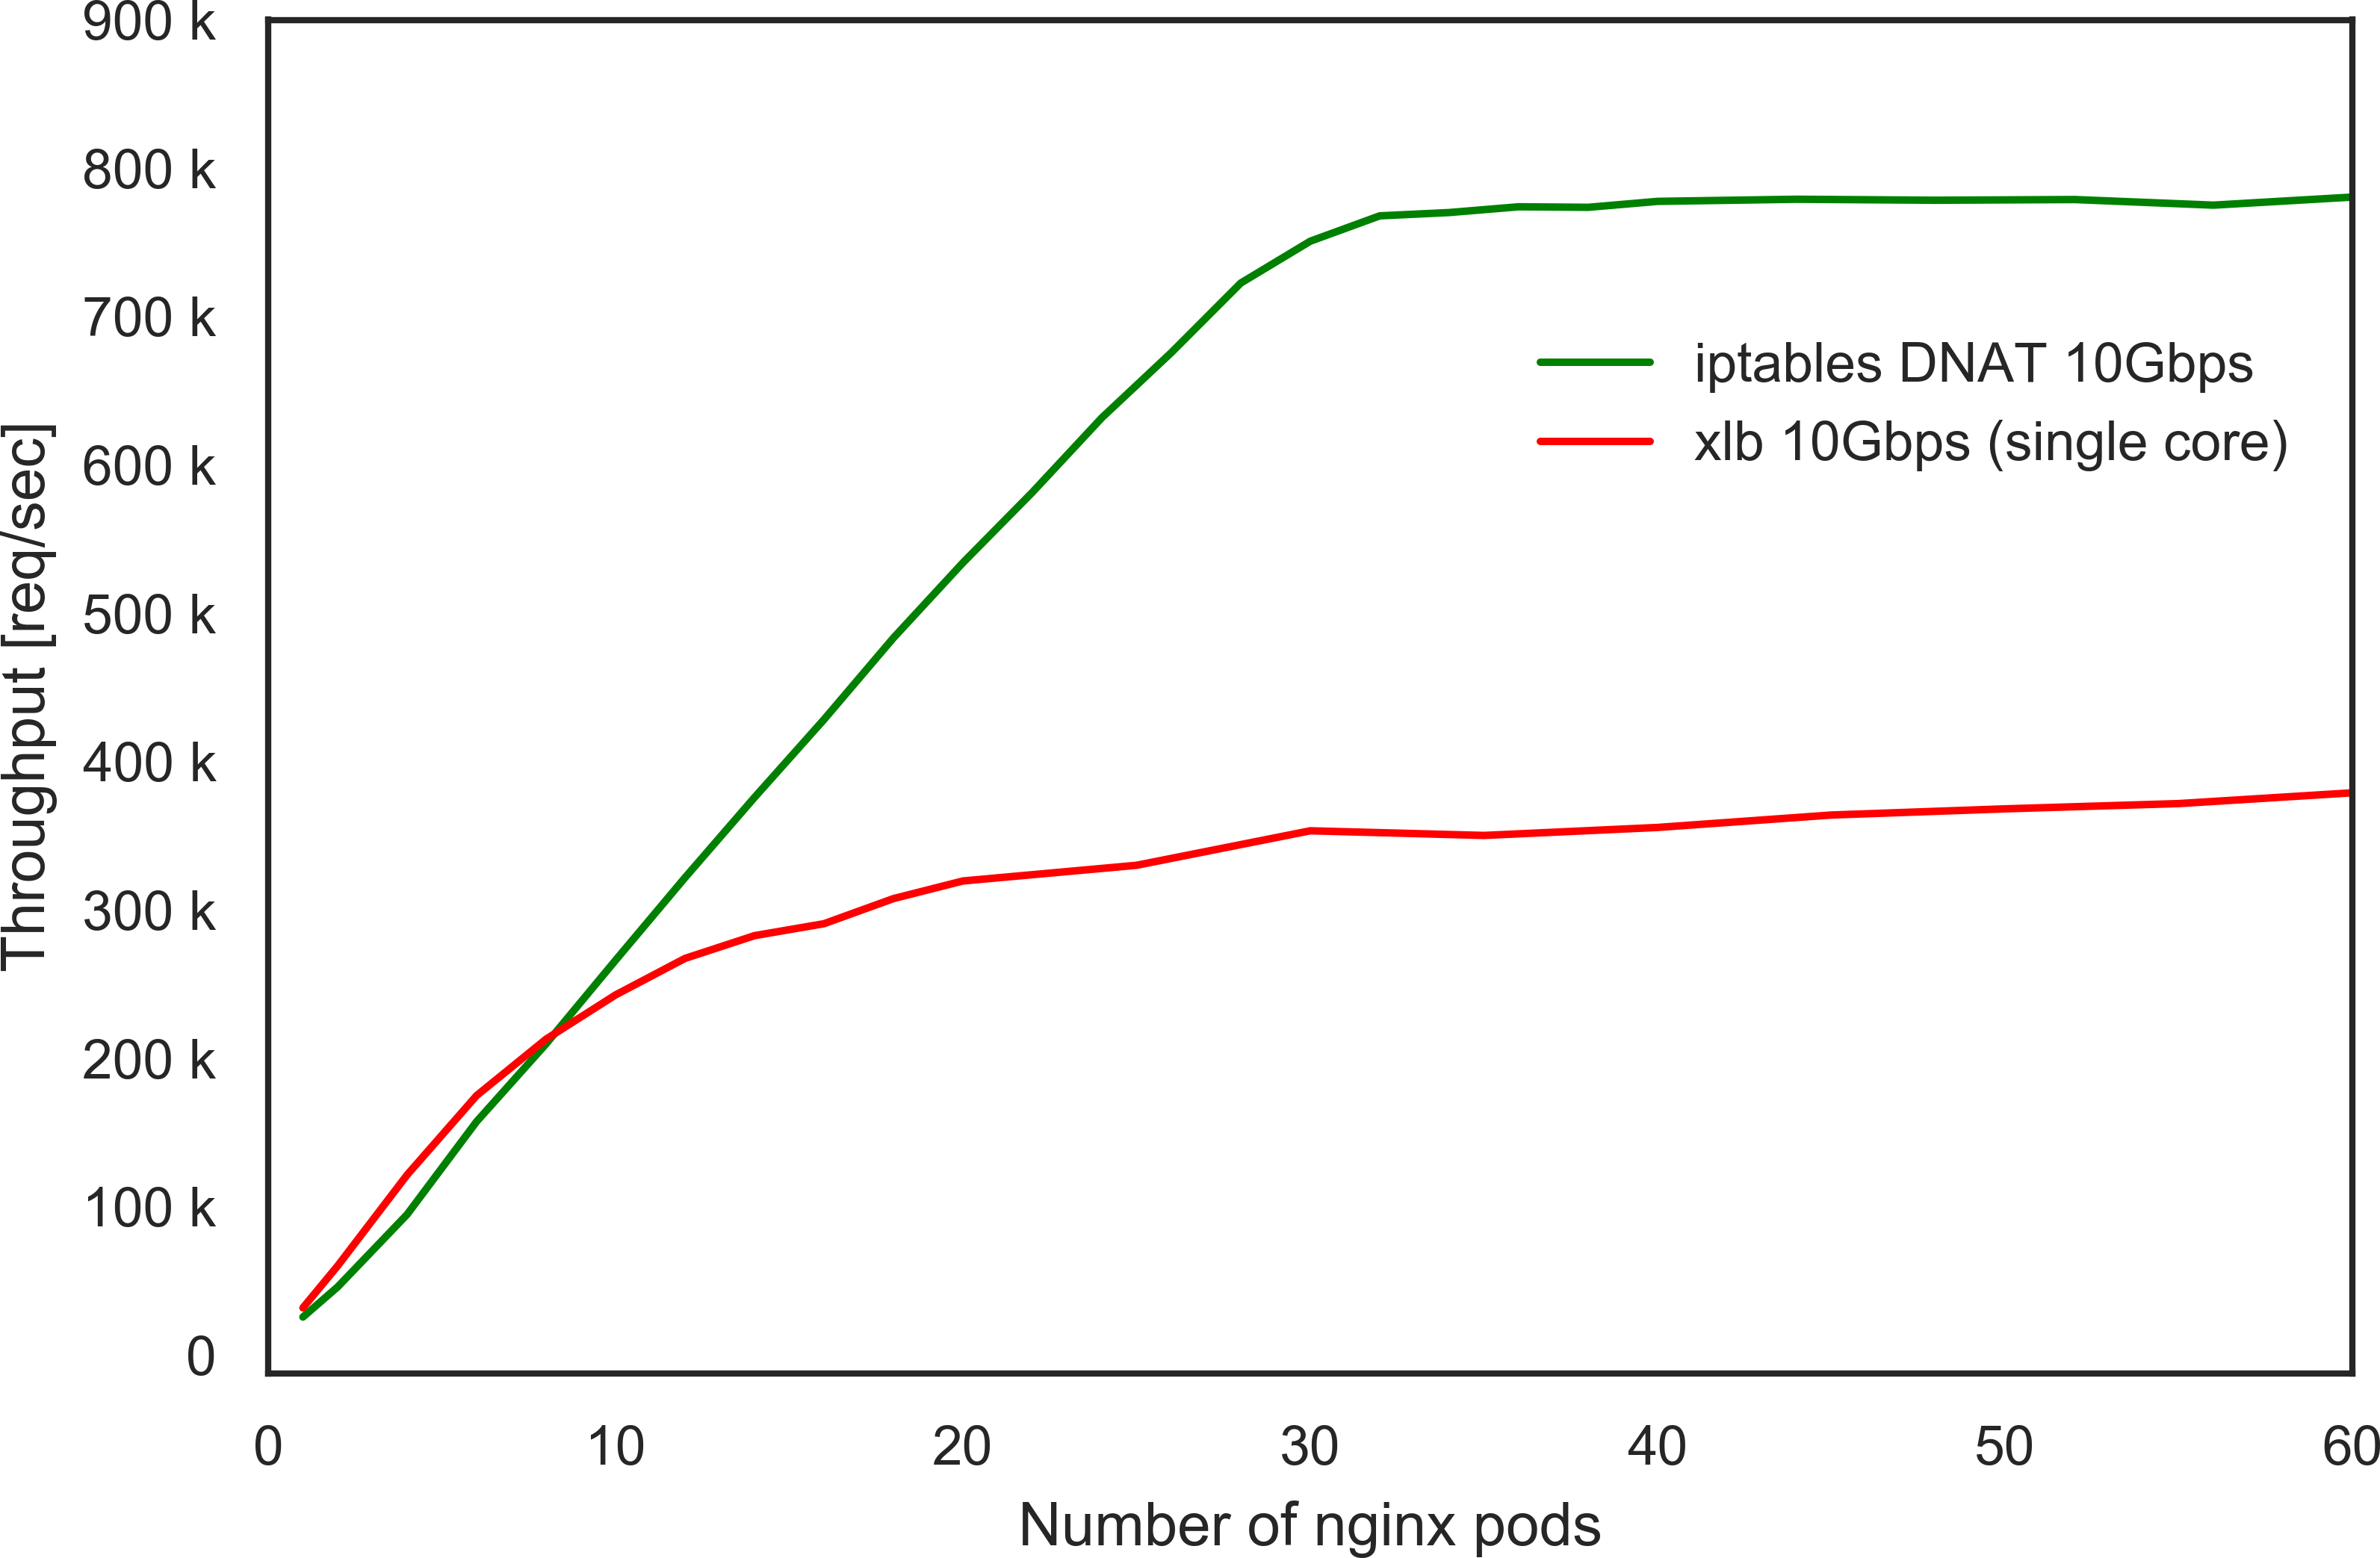
\includegraphics[width=0.9\columnwidth]{Figs/xlb_iptables_dnat_10g}
  \par\bigskip
  \centering
  \begin{minipage}{0.9\columnwidth}
    \caption[Throughput of xlb load balancer]{
      Throughput of xlb load balancer.
      The xlb load balancer is placed in node net namespace.
      The setting \enquote{(RSS,RPS)=(off,off)}, i.e., single core packet processing is used for the xlb measurement.
      The results of iptables DNAT for \enquote{(RSS,RPS)=(on,off)} and \enquote{(RSS,RPS)=(off,off)} are also shown for comparison.
      The throughput of the xlb is much higher than that of iptables DNAT with single core packet processing.
      Although using only a single core, the throughput of the xlb load balancer is close to half of the iptables DNAT's with 16 core (eight physical core) packet processing.
    }
    \label{fig:xlb_iptables_dnat_10g}
  \end{minipage}
\end{figure}

Figure~\ref{fig:xlb_iptables_dnat_10g} compares the throughput of xlb and iptables DNAT. 
Although a single core is used for the packet processing, the throughput of the xlb load balancer is 390k[req/sec], which is close to half of the iptables DNAT's throughput with 16 core (eight physical cores) packet processing.
Figure\ref{fig:cpu_usage_10g_xlb} compares CPU usages between xlb and iptables DNAT.
At a given throughput the xlb consumes much less CPU resource than iptables DNAT.
These results indicate that load balancer using XDP technology is very promising.


\begin{figure}[h]
  \centering
  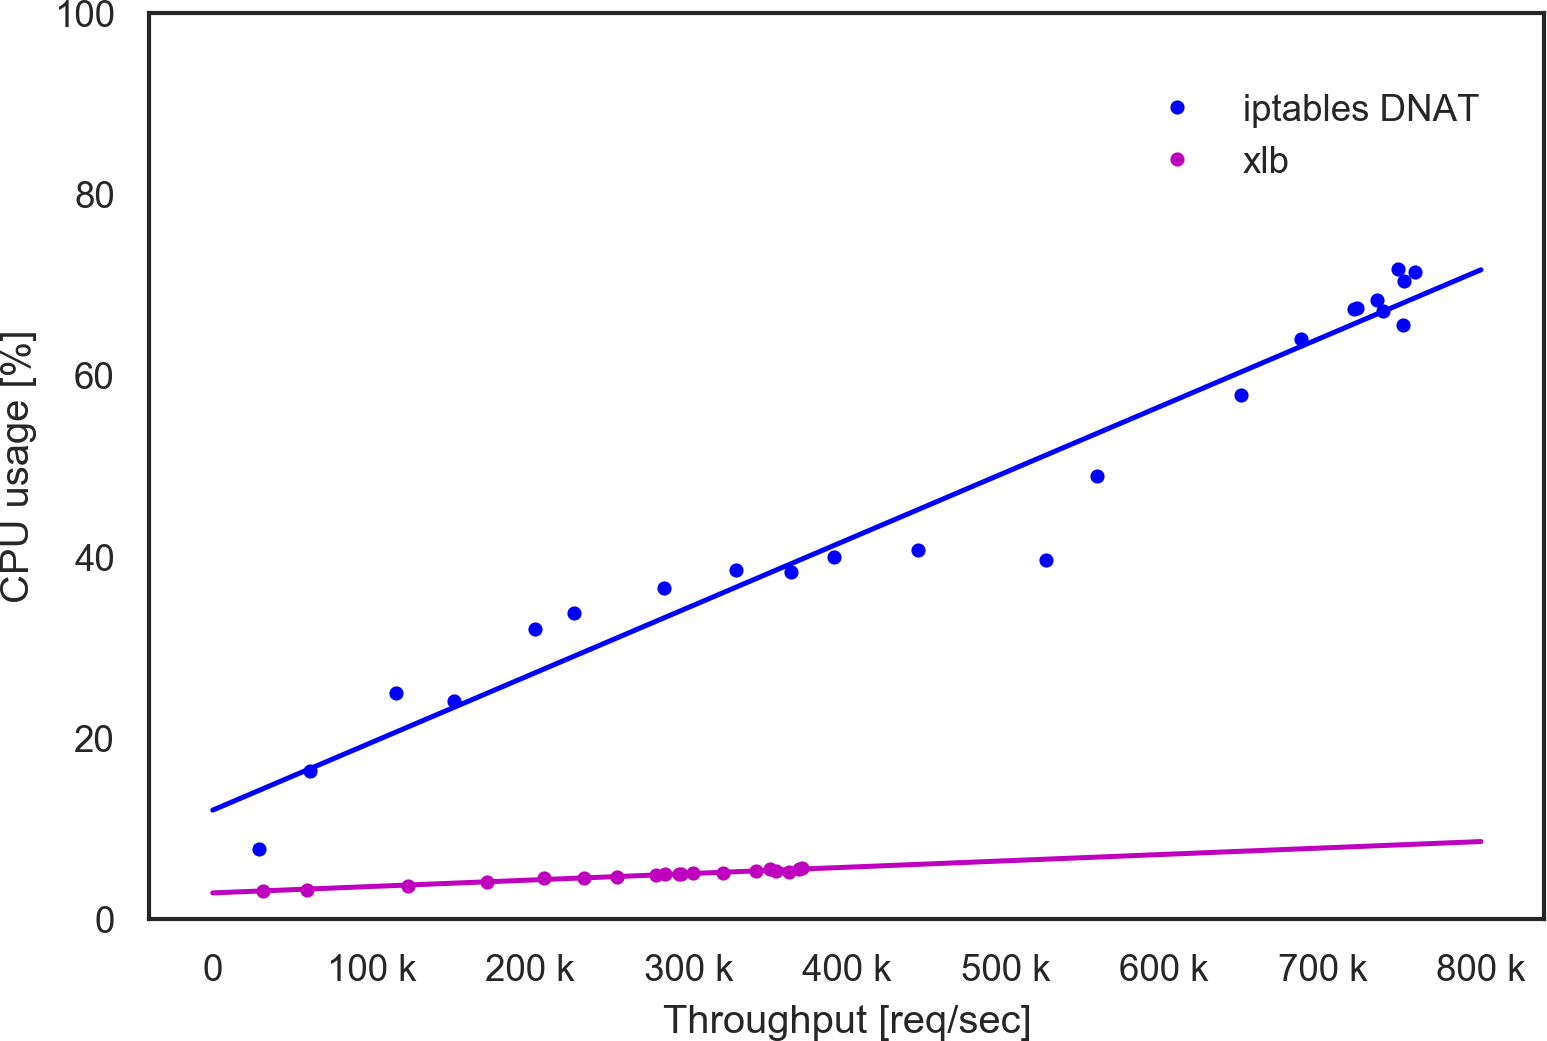
\includegraphics[width=0.9\columnwidth]{Figs/cpu_usage_10g_xlb}
  \par\bigskip
  \centering
  \begin{minipage}{0.9\columnwidth}
    \caption[CPU usage of xlb load balancer]{
      CPU usage of xlb load balancer.
      The xlb uses much less CPU resource than iptables DNAT.
    }
    \label{fig:cpu_usage_10g_xlb}
  \end{minipage}
\end{figure}

\FloatBarrier

\section{Summary}


In this chapter, the author has shown that the proposed load balancer has sufficient throughput in 10 Gbps network.
The maximum throughput for IPVS-TUN is 731K [req/sec], which is sufficient because four of the load balancers with ECMP setup can deal with maximum traffic of 2.9M [req/sec] in 10 Gbps network.



The author also discussed how to improve the performance levels for faster networks.
The throughputs of IPVS and IPVS-TUN in node net namespace are significantly improved from those in container net namespace.
This indicates that there is unignorable overhead due to container network using veth+bridge.
The CPU usage of the IPVS in node net namespace is more extensive than that of iptables DNAT, indicating that IPVS is inherently less efficient than iptables DNAT.
The author considers that both of these should be improved in future work.



As an effort to improve the efficiency of the software load balancer \added[id=5th]{itself}, 
the author has implemented a \added[id=5th]{novel} software load balancer, xlb, using XDP technology, and presented the preliminary experimental result.
The obtained throughput 390K [req/sec] with single core packet processing is very promising.
The author estimates that about five of the software load balancer using this technology with 16 core packet processing can provide sufficient throughput, 29M [req/sec] in 100 Gbps environments in the future. 


From these results, the author concludes this chapter as follows;
1) The proposed load balancer has sufficient performance levels in 10 Gbps network environment.
2) For a faster network, e.g., 100 Gbps, improvement in container network and in software load balancer itself is needed, which should be explored in future work.
3) The author implemented a software load balancer using XDP technology, and the preliminary result has shown that this technology is very promising.

